% Chapter Template

\chapter{Diseño} % Main chapter title

\label{Chapter4} % Change X to a consecutive number; for referencing this chapter elsewhere, use \ref{ChapterX}

\lhead{Capítulo  4. \emph{Diseño}} % Change X to a consecutive number; this is for the header on each page - perhaps a shortened title

%----------------------------------------------------------------------------------------
%	SECTION 1
%----------------------------------------------------------------------------------------
\section{Dominio del Problema}
Como se detalló en la Sección ~\ref{section:controladores} todos los cerramientos eléctricos no funcionan por sí solos sino que necesitan de un controlador. Estos controladores se comercializan en diferentes presentaciones con distintos diseños, desde simples interfaces eléctricas para un botón pulsador externo como se muestra en la Figura ~\ref{fig:controladoras_simple_compleja}(a) hasta complejas centrales de acceso electrónico como la que se muestra en la Figura ~\ref{fig:controladoras_simple_compleja}(b) que incluyen interfaces para sistemas de identificación de usuarios o soporte para llaves electrónicas descritas en la Sección ~\ref{section:llaves_electronicas}.
\begin{figure}[htbp]
	\centering
	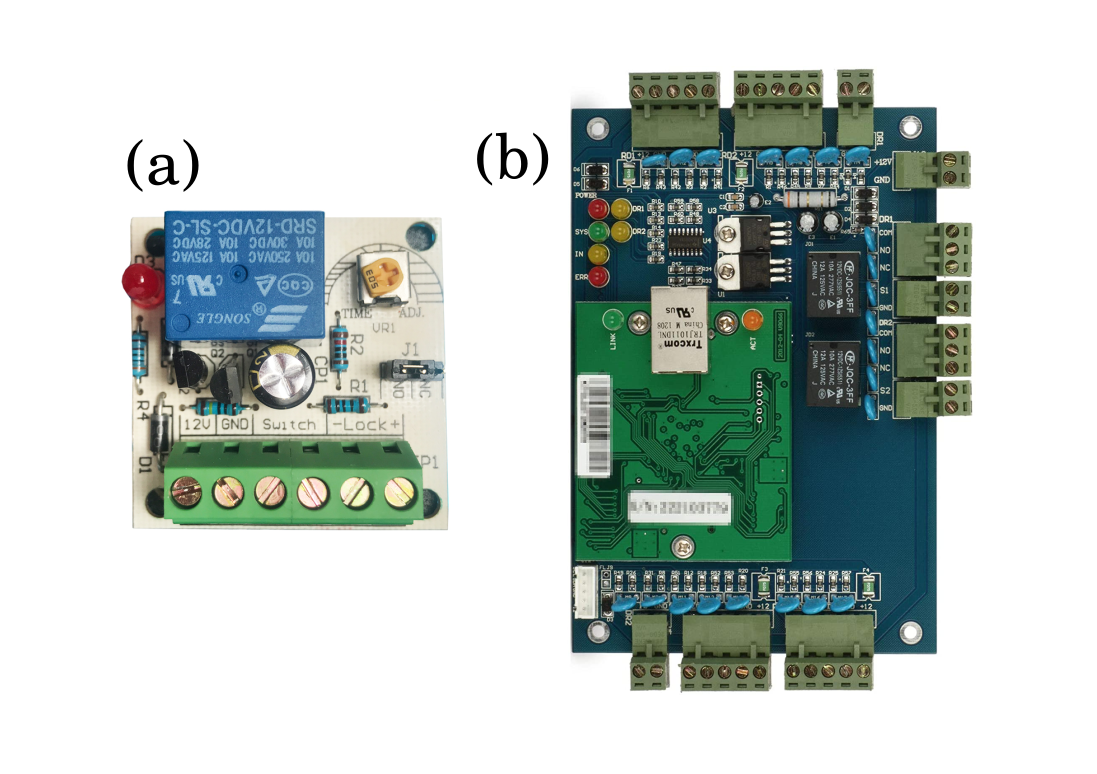
\includegraphics[width=0.6\textwidth]{Pictures/controladoras_simple_compleja.png}
	\rule{35em}{1pt}
	\caption[Controladoras Comparativa]{Controladoras de cerramientos eléctrico, a la izquierda un simple adaptador de voltaje a la derecha una central de acceso con múltiples puertos. }
	\label{fig:controladoras_simple_compleja}
\end{figure}
\subsection{Conexión con los controladores}
Del análisis y la comparación de los distintos tipos de controladores se pudo inferir el diseño general de estos sistemas así como sus componentes principales y accesorios que se listan a continuación:\\
\textbf{PRINCIPALES}
\begin{itemize}
	\item Etapa de Potencia y Adaptación de Voltajes 
	\item Driver Señal de Cerramiento
	\item Borneras para Cerramientos
	\item Bornera Pulsador Externo
	\item Microcontrolador y Firmware
\end{itemize}
\textbf{ACCESORIOS}
\begin{itemize}
	\item Bornera Luz Testigo Externa
	\item Bornera Barrera Infrarroja
	\item Bocina
	\item LEDs de Funcionamiento
	\item Pantalla
	\item Teclado
	\item Conmutadores Deslizantes de Configuración (DIP Switch)
	\item Jumpers de Configuración
	\item Pulsadores de Configuración
	\item Sensores Funcionamiento y Estado
	\item Módulo portero telefónico o Intercom
	\item Módulo RX RF para control remoto
	\item Lector etiquetas RFID
	\item Sensor Huella dactilar
\end{itemize}
En la Figura ~\ref{fig:controller_bdd} se puede observar un diagrama de definición por bloques del diseño generalizado para las controladoras de cerramientos eléctricos. Se resalta en violeta el componente correspondiente el pulsador físico externo.\\
\begin{figure}[htbp]
	\centering
	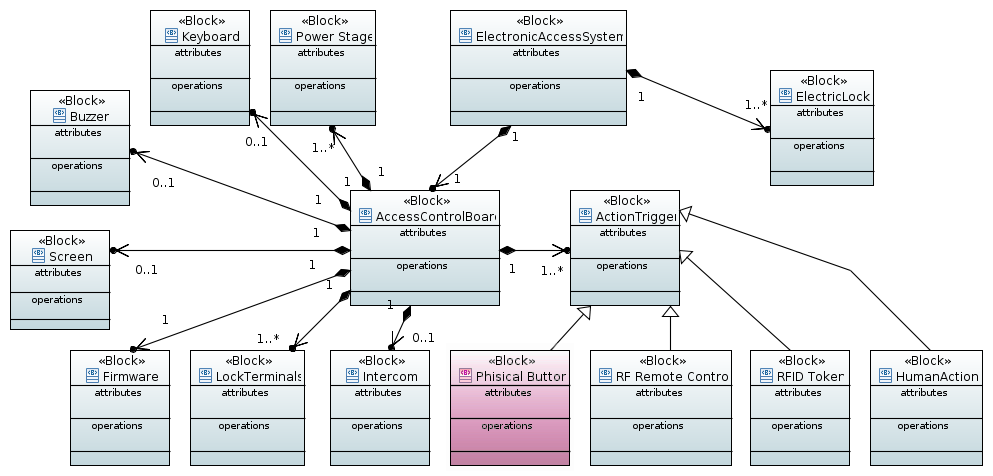
\includegraphics[width=0.9\textwidth]{Pictures/controller_bdd.png}
	\rule{35em}{1pt}
	\caption[Diagrama Bloques Controlador]{Diagrama de definición por bloques para la generalización del diseño de los controladores.}
	\label{fig:controller_bdd}
\end{figure}
En el diagrama de bloques interno del controlador de la Figura ~\ref{fig:ibd_controladora} la señal de activación del pulsador es procesada por el módulo de disparador de acciones en la mayoría de los casos generando la señal de apertura o cierre del cerramiento según sea el estado del mismo.\\
\begin{figure}[htbp]
	\centering
	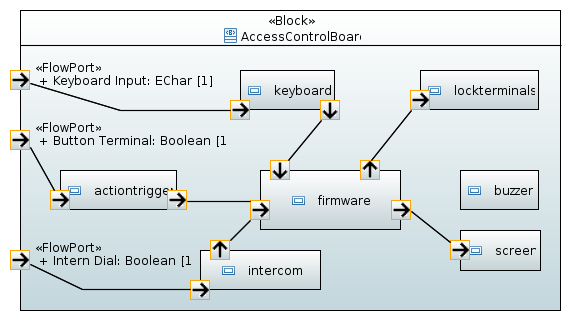
\includegraphics[width=0.6\textwidth]{Pictures/IBD_controladora.png}
	\rule{35em}{1pt}
	\caption[Diagrama Bloques Internos Controlador]{Diagrama de bloques internos del diseño generalizado de un controlador de cerramientos eléctricos.}
	\label{fig:ibd_controladora}
\end{figure}
Después de realizar el análisis de los diseños se pudo evidenciar que la bornera para pulsador o botón externo es un factor común entre todos los modelos. Teniendo en cuenta esta particularidad se decidió adoptar esta interfaz de accionamiento como el modo de conexión universal de la solución a ser implementada. En la Figura ~\ref{fig:componentes_controladora+sol} se muestra un diagrama de componentes de alto nivel dónde se ilustra tal decisión.
\begin{figure}[htbp]
	\centering
	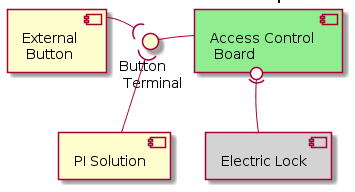
\includegraphics[width=0.5\textwidth]{Pictures/componentes_controladora+sol.png}
	\rule{35em}{1pt}
	\caption[Diagrama de Componentes Conexión al Controlador]{Diagrama de componentes de alto nivel muestra la conexión propuesta para la solución de hardware.}
	\label{fig:componentes_controladora+sol}
\end{figure}
\subsection{Funcionalidades básicas de un Sistema de Acceso}
Estos sistemas ofrecen la posibilidad de limitar el acceso a ciertas áreas de un inmueble mediante el control de cerramientos eléctricos utilizando llaves electrónicas u otros modos de autenticación de usuarios como sensores biométricos o el ingreso de credenciales por teclados. Para poder llevar a cabo esta tarea es primordial que estos controladores implementen una interfaz de configuración que permita entre otras operaciones:
\begin{itemize}
	\item Permitir la configuración del sistema utilizando una clave maestra.
	\item Dar de alta llaves electrónicas, nuevas credenciales biométricas o por teclado.
	\item Dar de baja llaves electrónicas, credenciales biométricas o por teclado.
	\item Resetear el sistema a sus valores de fábrica.
\end{itemize}
\section{Requerimientos}
Considerando las funcionalidades básicas de un sistema de acceso tradicional y el modo de conexión universal elegido se listan a continuación los requerimientos a nivel sistema de la solución propuesta.
\subsection{Requerimientos a nivel de Sistema}
A nivel de sistema se listan los requerimientos identificados en la Tabla ~\ref{table:req_sistemas}.
\begin{table}[ht]
	%\centering
	%\resizebox{\textwidth}{!}{
		\begin{tabular}{|l|m{12cm}|}
			\hline
			\textbf{ID} & \textbf{Descripción}                                                                                             \\ \hline
			RS00        & El sistema debe accionar cerramientos eléctricos.                                                                \\ \hline
			RS01        & El sistema debe permitir que un mismo usuario tenga acceso a múltiples cerramientos.                             \\ \hline
			RS02        & El sistema debe establecer conexión a la red wifi del inmueble donde será instalado.                             \\ \hline
			RS03        & El sistema debe mantenerse operativo offline de manera local.                                                    \\ \hline
			RS04        & El sistema debe funcionar de manera remota a través de internet.                                                 \\ \hline
			RS05        & El sistema debe admitir alta de nuevos usuarios para un cerramiento.                                             \\ \hline
			RS06        & El sistema debe permitir la baja de usuarios.                                                                    \\ \hline
			RS07        & El sistema debe permitir el cambio de privilegios de los usuarios.                                               \\ \hline
			RS08        & El sistema debe admitir la conexión y calibración de sensores (fin de carrera, encoder y de apertura magnética). \\ \hline
			RS09        & El sistema debe permitir su restablecimiento a valores de fábrica.                                               \\ \hline
			RS10        & El sistema debe permitir actualizar su versión de software de manera sencilla.                                   \\ \hline
		\end{tabular}
	%}
	\caption[Requerimientos de Sistema]{Tabla de requerimientos a nivel de sistema para la solución propuesta.}
	\label{table:req_sistemas}
\end{table}
\subsection{Requerimientos del Módulo Electrónico}
Los requerimientos encontrados para el Módulo Electrónico se listan en la Tabla ~\ref{table:req_modulo_electro}.
Estos requerimientos fueron implementados por un colaborador del equipo quién se encargó principalmente del desarrollo de firmware por lo que los detalles del diseño y la implementación del software embebido quedan fuera del presente informe. 
\begin{table}[ht]
	%\centering
	%\resizebox{\textwidth}{!}{
		\begin{tabular}{|c|m{12cm}|}
			\hline
			\textbf{ID} & \multicolumn{1}{c|}{\textbf{Descripción}}                                                                                    \\ \hline
			RME00       & El módulo electrónico debe alimentarse con 220v AC.                                                                          \\ \hline
			RME01       & El módulo electrónico debe conectarse al controlador por la bornera de pulsador externo                                      \\ \hline
			RME02       & El módulo electrónico debe conectarse a la red wifi del inmueble donde será instalado.                                       \\ \hline
			RME03       & El módulo electrónico debe almacenar los usuarios registrados autorizados para                                               \\ \hline
			RME04       & El módulo electrónico debe funcionar de manera remota a través de internet.                                                  \\ \hline
			RME05       & El módulo electrónico debe funcionar de manera local offline en caso de que la conexión a internet se vea interrumpida.      \\ \hline
			RME06       & El módulo electrónico debe recibir comandos desde la aplicación cliente y devolver una respuesta según se detalla en la API. \\ \hline
			RME07       & El módulo electrónico debe contar con puertos para los distintos tipos de sensores.                                          \\ \hline
			RME08       & El módulo electrónico debe contar con luces indicadoras de funcionamiento.                                                   \\ \hline
			RME09       & El módulo electrónico debe incluir botones para configuración y operación.                                                   \\ \hline
			RME10       & El módulo electrónico debe poder actualizar su versión de firmware de manera inalámbrica.                                    \\ \hline
		\end{tabular}
	%}
	\caption[Requerimientos del Módulo Electrónico]{Tabla de requerimientos del Módulo Electrónico.}
	\label{table:req_modulo_electro}
\end{table}
\subsection{Requerimientos de la Aplicación}

\begin{table}[ht]
	%\centering
	%\resizebox{\textwidth}{!}{
		\begin{tabular}{|l|m{12cm}|}
			\hline
			\multicolumn{1}{|c|}{\textbf{ID}} & \multicolumn{1}{c|}{\textbf{Descripción}}                                                                 \\ \hline
			RA00                              & La aplicación debe permitir el registro inicial del usuario con su número de teléfono.                    \\ \hline
			RA01                              & La aplicación debe generar una clave única y secreta para el envío de comandos.                           \\ \hline
			RA02                              & La aplicación debe descubrir y listar módulos electrónicos nuevos y ya configurados.                      \\ \hline
			RA03                              & La aplicación debe permitir enviar comandos al módulo y recibir la respuestas según se detalla en la API. \\ \hline
			RA04                              & La aplicación debe permitir configurar los módulos nuevos.                                                \\ \hline
			RA05                              & La aplicación debe permitir solicitar acceso a los módulos electrónicos encontrados ya configurados.      \\ \hline
			RA06                              & La aplicación debe permitir el accionamiento de los cerramientos eléctricos.                              \\ \hline
			RA07                              & La aplicación debe permitir cambiar el alias de los módulos.                                              \\ \hline
			RA08                              & La aplicación debe ofrecer un modo de accionamiento con pantalla bloqueada.                               \\ \hline
			RA09                              & La aplicación debe ofrecer distintas configuraciones según el privilegio del usuario.                     \\ \hline
			RA10                              & La aplicación debe permitir al usuario administrador restablecer el módulo a valores de fábrica.          \\ \hline
			RA11                              & La aplicación debe permitir al usuario administrador calibrar el sensor.                                  \\ \hline
			RA12                              & La aplicación debe permitir al usuario administrador invitar a nuevos usuarios.                           \\ \hline
			RA13                              & La aplicación debe permitir al usuario administrador convertir usuarios a administradores.                \\ \hline
			RA14                              & La aplicación debe permitir al usuario administrador eliminar cualquier usuario.                          \\ \hline
			RA15                              & La aplicación debe permitir al usuario administrador actualizar la versión del firmware del módulo.       \\ \hline
		\end{tabular}
	\caption[Requerimientos de la Aplicación]{Tabla de requerimientos de la Aplicación Cliente.}
	\label{table:req_aplicacion}
%	}
\end{table}

\section{Gestión de Riesgos}
En esta sección se expone el panorama de incertidumbres del proyecto y se hace foco en las eventualidades que pueden surgir durante su ejecución que pueden alterar de alguna manera la planificación y duración del proyecto.
La gestión temprana de riesgos facilita la identificación de los mismos y permite la creación de planes de contingencia para minimizar el efecto en caso de ocurrencia.

\subsection{Identificación de Riesgos}
Las situaciones que puedan constituir una amenaza a la realización del proyecto se pueden clasificar por el objeto de impacto o por su causalidad.

Categorización por objeto de impacto.
\begin{itemize}
	\item Al Proyecto: afectan la planificación y los recursos del proyecto.
	\item Al Producto: afectan la calidad o el rendimiento del producto.
	\item Al Negocio: afectan a la organización que desarrolla el producto.
\end{itemize}


Por otro lado se pueden clasificar los riesgos respecto de su origen o causa.

\begin{itemize}
	\item \textbf{Riesgo Tecnológico} (TECNO): Estrechamente relacionado con los aspectos técnicos del proyecto se evidencian en las herramientas utilizadas para la implementación, evaluación y ejecución del trabajo. En el caso del presente proyecto existirán riesgos de hardware y software.
	\item \textbf{Riesgo de Personal} (PER) : Relacionados a las personas involucradas en la ejecución del proyecto. En este caso el equipo de desarrollo.
	\item \textbf{Riesgo Organizacional}(ORG): Derivan del entorno dónde se está realizando el trabajo. En este caso el proyecto está vinculado a un emprendimiento tecnológico.
\end{itemize}

\subsection{Análisis de Riesgo}
Para poder tener un panorama completo de los riesgos del proyecto se elabora una tabla con los riesgos identificados y se pondera de manera cualitativa los mismos. Los parámetros de esta ponderación serán la probabilidad de ocurrencia y el impacto de su efecto.\\
\textbf{La probabilidad de ocurrencia} se estimará en tres valores: Improbable (0.3), Probable (0.6) y Muy Probable (0.9).\\
\textbf{El impacto} se estimará también en tres valores: Bajo (1), Moderado(10), Alto(100)\\
Realizando el producto aritmético entre estos parámetros se calcula la importancia de los riesgos identificados como se puede observar en la Tabla ~\ref{table:riegos_identificados}.
Aunque el valor de importancia obtenido es ilustrativo ofrece una alternativa numérica que permite el ordenamiento y con esto un inmediato orden de prioridad.

\begin{table}[ht]
	%\centering
	%\resizebox{1\textwidth}{!}{
		\begin{tabular}{|c|m{3cm}|m{5em}|c|c|c|c|}
			\hline
			\textbf{ID} & \multicolumn{1}{c|}{\textbf{Descripción}}                                        & \textbf{Objeto de Impacto} & \textbf{Causa} & \textbf{Probabilidad} & \textbf{Impacto} & \textbf{Importancia} \\ \hline
			R00         & Problemas con el entendimiento de la arquitectura elegida para la implementacion & PROY                       & PER            & 0.3                   & 100              & 30                   \\ \hline
			R01         & Implementación de la arquitectura elegida                                        & PROY                       & PER            & 0.6                   & 100              & 60                   \\ \hline
			R02         & Entendimiento del paradigma de programacion reactiva utilizando RxJava           & PROY                       & PER            & 0.6                   & 10               & 6                    \\ \hline
			R03         & Cambio de versiones de librerias                                                 & PROY                       & TEC            & 0.6                   & 1                & 0.6                  \\ \hline
			R04         & Falta de librerías de comunicacion                                               & PROY                       & TEC            & 0.3                   & 100              & 30                   \\ \hline
			R05         & Librerias de comunicacion no adaptadas a programacion reactiva                   & PROY                       & TEC            & 0.6                   & 10               & 6                    \\ \hline
			R06         & Falta de documentación de las librerías                                          & PROY                       & TEC            & 0.9                   & 10               & 9                    \\ \hline
			R07         & Retraso o complicaciones en el desarrollo del módulo electrónico                 & PROY                       & PER            & 0.9                   & 100              & 90                   \\ \hline
			R08         & Subestimación de tiempo de desarrollo                                            & PROY                       & ORG            & 0.9                   & 10               & 9                    \\ \hline
			R09         & Cambio de requerimientos durante el deesarrollo                                  & PROY                       & NEG            & 0.9                   & 100              & 90                   \\ \hline
		\end{tabular}
	\caption[Riesgos Identificados]{Tabla de riesgos identificados y la ponderación para el cálculo de su importancia.}
	\label{table:riegos_identificados}
%	}
\end{table}

\subsection{Planificación de Riesgos}
Con el objetivo de minimizar los efectos de las posibles eventualidades riesgosas se plantean tres tipos de estrategias que se detallan a continuación.

\begin{itemize}
	\item De Prevención: Acciones preventivas orientadas a reducir la probabilidad de ocurrencia.
	\item De Mitigación: Acciones preventivas orientadas a atenuar el impacto en caso de ocurrencia.
	\item De Contingencia: Acciones curativas en caso de ocurrencia.
\end{itemize}

Para los 5 riesgos identificados más importantes se plantearon las estrategias y se exponen en la Tabla ~\ref{table:planificacion_riesgos}.

\begin{table}[ht]
	%\centering
	%\resizebox{1\textwidth}{!}{
	\begin{tabular}{|c|m{3cm}|m{3cm}|m{3cm}|m{3.5cm}|}
		\hline
		\multirow{2}{*}{\textbf{ID}} & \multicolumn{1}{c|}{\multirow{2}{*}{\textbf{Descripción}}}                       & \multicolumn{3}{c|}{\textbf{Estrategia}}                                                                                                                                                                                                                                                                                                                                                                                                                                                                                           \\ \cline{3-5} 
		& \multicolumn{1}{c|}{}                                                            & \multicolumn{1}{c|}{\textbf{De Prevención}}                                                                                                                           & \multicolumn{1}{c|}{\textbf{De Mitigación}}                                                                                                                                  & \multicolumn{1}{c|}{\textbf{De Contingencia}}                                                                                                                               \\ \hline
		R06                          & Retraso o complicaciones en el desarrollo del módulo electrónico                 & Se iniciará el desarrollo de ambos componentes una vez que se hayan establecido las tecnologías para ambos.                                                           & Se establecerá con claridad una API de comunicación a modo de contrato y con una versión definida.                                                                           & Con las definiciones de la API se puede simular el comportamiento del módulo.                                                                                               \\ \hline
		R08                          & Cambio de requerimientos durante el desarrollo                                  & Se celebraran entrevistas con los posibles clientes y usuarios para anticipar cambios y requerimientos futuros.                                                       & Se realizará una revisión de los requerimientos periódica.                                                                                                                   & Se planificará la modificación o adición de funcionalidad para la próxima versión. Intentando mantener siempre un entregable funcional.                                       \\ \hline
		R01                          & Implementación de la arquitectura elegida                                        & Se buscarán ejemplos de implementaciones similares y documentación respaldatoria.                                                                                     & Se contará con el apoyo de algún contacto técnico externo con experiencia para poder consultar.                                                                              & Se agregarán la resolución de conflictos a la planificación de tareas ordinarias para tener en cuenta el impacto y el progreso en ese aspecto.                              \\ \hline
		R00                          & Problemas con el entendimiento de la arquitectura elegida para la implementación & Se recolectará bibliografía diversa sobre los conceptos introducidos con la arquitectura.                                                                             & Se podrá realizar consultas inter-equipo para despejar dudas y evitar retrasos.                                                                                              & Se pondrá en marcha un pequeño análisis de impacto al reemplazar el asunto bloqueante por una alternativa más sencilla y quedará documentado.                               \\ \hline
		R03                          & Falta de librerías de comunicación                                               & Se escogerá un framework de desarrollo lo suficientemente maduro como para anticipar la búsqueda de las librerías necesarias. Y asegurar la existencia de las mismas. & Se empleará un modo de implementación por interfaces a modo Mock, de manera que se pueda postergar el uso de la biblioteca sin retrasar el desarrollo de las funcionalidades & Se buscarán alternativas a los protocolos originalmente propuestos y se evaluará el impacto sobre la implementación. En caso de ser un cambio viable se dejará documentado. \\ \hline
	\end{tabular}
	\caption[Planificación de Riesgos]{Tabla con la planificación de los riesgos más importantes.}
	\label{table:planificacion_riesgos}
%}
\end{table}
 


